
\noindent Today we will use Sloan Digital Sky Survey images
to investigate the deep sky. These are similar to the Palomar prints
used earlier. However, they are deeper and higher resolution, and
taken with more modern equipment (precision digital cameras instead of
photographic plates). Unlike the Palomar prints, which were single
photographic images, these images are many small images stitched
together digitally. 

Recall that the images are negatives so the light of the stars etc. is
dark. Pick one of the available pairs supplied by your instructors.

{\bf Please treat them with great care: keep them flat; no pencils or
pens or food near them, and do not write on paper on top of the
prints. Thanks!}

\noindent
{\bf 1. The Virgo Cluster of galaxies:} 

\noindent Look at the image marked for RA$=12$h,
Dec$=+11^\circ$. Notice that there are a lot of big galaxies in the
image! This is the Virgo Cluster of galaxies.  Why is it so called?

\vspace{20pt}

\noindent The Virgo Cluster is known to be about 60 Mlyrs away.
Assume that this 3 by 3 degree field covers most of it.  What is its
approximate size?

\vspace{40pt}

\noindent Count how many objects are greater than about 40 thousand
lightyears in diameter in the image. Note there are many many more
smaller galaxies!

\vspace{40pt}

\noindent Find this field in Starry Night.  What is the name of the
brightest galaxy in the cluster?

\vspace{20pt}

\noindent
{\bf 2. Merging galaxies}

\noindent Find the close pair of galaxies about 1 deg East of the
center. These galaxies are {\it merging} with each other.  In a few
hundred million years they will be a single galaxy.  Estimate the
separation between the two components.

\vspace{40pt}

\noindent Find the close pair about 2 deg North-Northwest of the
center. Look at it through the magnifying class, and draw it below.

\clearpage

\noindent 
{\bf 3. Galaxy types}

\noindent In the figure at the end of lab there is a version of the
classical ``Hubble tuning fork'' used to classify galaxies.
``Elliptical galaxies'' are on the left and ``spirals'' are on the
right.  What type of galaxy is the very bright one a little North of
center? What type of galaxy is the bright one near the bottom edge,
left of center? Can you find a ``barred'' galaxy? 

\vspace{40pt}

\noindent Why do you suppose some galaxies are very ``flat'' and some
look like circles?

\vspace{40pt}

\noindent 
{\bf 4. Galaxy colors}

\noindent Look up this location using {\tt http://skyserver.sdss.org} on your
browser. Find some spiral galaxies in the field, and find some
elliptical galaxies in the field.  Which ones are redder and which
ones are bluer? Why do you suppose that is?

\vspace{40pt}

\noindent 
{\bf 5. The Hercules cluster}

\noindent Look at the other image, this one at RA$=16$h,
Dec$=+17^\circ$. There is another cluster in this image: can you find
it? Use the magnifying glass to make sure you are looking at a cluster
of galaxies. This is a very large nearby cluster, among the largest of
about 4000 clusters that George Abell published in 1958 based on
staring by eye at Palomar observations of this field. 

\noindent Assuming that this cluster is the same physical size as
Virgo, estimate its distance. 

\vspace{40pt}

\noindent Look carefully at the galaxies with the magnifying glass?
How many can you find that appear to be merging?

\vspace{40pt}

\clearpage

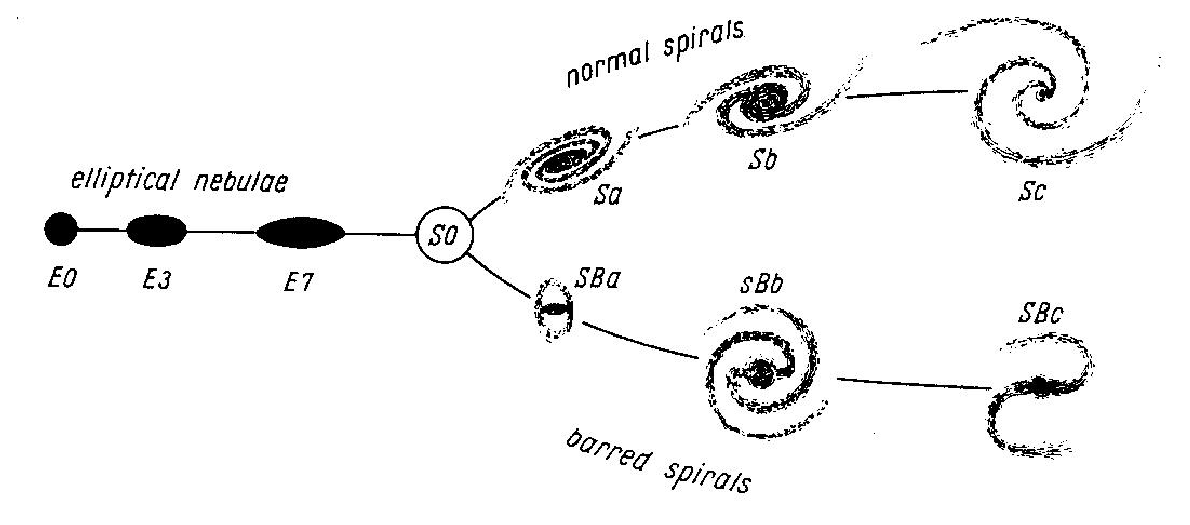
\includegraphics[width=5.5in]{tune.eps}
